% arara: pdflatex
% arara: bibtex
% arara: pdflatex
% arara: pdflatex
\documentclass[10pt,twocolumn,letterpaper]{article}

\usepackage{cvpr}
\usepackage{times}
\usepackage{epsfig}
\usepackage{graphicx}
\usepackage{amsmath}
\usepackage{amssymb}
\usepackage{pdfpages}
\usepackage{caption}
\usepackage{subcaption}

% Include other packages here, before hyperref.

% If you comment hyperref and then uncomment it, you should delete
% egpaper.aux before re-running latex.  (Or just hit 'q' on the first latex
% run, let it finish, and you should be clear).
\usepackage[breaklinks=true,bookmarks=false]{hyperref}

\cvprfinalcopy % *** Uncomment this line for the final submission

\def\cvprPaperID{****} % *** Enter the CVPR Paper ID here
\def\httilde{\mbox{\tt\raisebox{-.5ex}{\symbol{126}}}}

% Pages are numbered in submission mode, and unnumbered in camera-ready
%\ifcvprfinal\pagestyle{empty}\fi
\setcounter{page}{1}

%%%%%%%%% TITLE
\title{Depth-Preserving Style Transfer}

\author{Xiuming Zhang\\
MIT CSAIL\\
{\tt\small xiuming@mit.edu}\\
\\
Teammates: Ruizhi Liao \& Yu Xia
}

\begin{document}

\makeatletter
\let\@oldmaketitle\@maketitle% Store \@maketitle
\renewcommand{\@maketitle}{\@oldmaketitle% Update \@maketitle to insert...
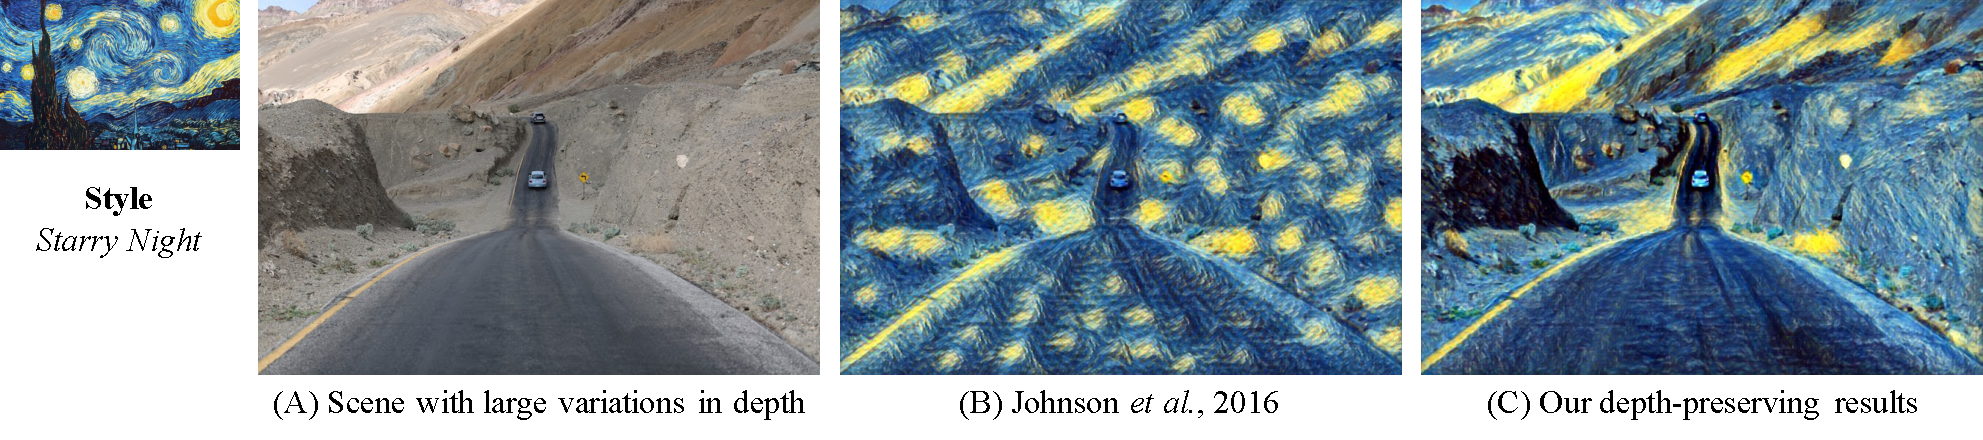
\includegraphics[width=\linewidth]{results/teaser.pdf}
When the input scene exhibits large variations in depth (A), the current state of the art tends to destroy the layering and lose the depth variations, producing a ``flat'' stylization result (B). This paper aims to address this issue by incorporating depth preservation into the loss function such that variations in depth and layering are preserved in the stylized image (C). 
\bigskip}
\makeatother

\maketitle
%\thispagestyle{empty}

%%%%%%%%% ABSTRACT
\begin{abstract}
Style transfer is defined as the process that given a content image and a style image it tries to migrate the style from the style image to the content image. Though it is not clear what the exact definition of style is, pattern transforming and matching are generally accepted.

In this work we present a novel method which preserve the depth information of the content image while migrating the style.
\end{abstract}

%%%%%%%%% BODY TEXT

\section{Introduction}

Deep neural networks have gained much popularity in a wide range of computer vision tasks, from low-level tasks, such as image denoising~\cite{xie2012image} and sharpening, to mid-level tasks, such as keypoint detection~\cite{sun2013deep}, to high-level tasks, such as object recognition~\cite{krizhevsky2012imagenet}. Besides supervised tasks with ground truth of training data available (such as scene classification), deep neural networks are also capable of solving more abstract problems, where no ground truth exists for training data. Image style transfer---the process of applying the style of a style input image (\eg, Van Gogh's \textit{Starry Night}) to a content input image---is one such task, because there exists no ``ground-truth stylization'' for any given content input image. 

Deep neural networks' capability of performing image style transfer was first demonstrated by~\cite{gatys2016image}, where neural networks are used to both transform images and compute loss. Under this optimization framework, the image transform network iteratively updates its output so that its content loss and style loss are minimized. This approach produces visually pleasant results, but suffers from slow performance due to its iterative nature. To address this issue, Johnson \etal~\cite{johnson2016perceptual} trains a residual neural network~\cite{he2016deep} that, once trained, only needs a feed-forward pass to stylize an input image. Although this method significantly reduces computational burden as compared with~\cite{gatys2016image}, it is unable to preserve the content image's variations in depth during style transfer (teaser figure B), hence destroying the sense of layering.

Although crucial to human perception and aesthetic sense, depth preservation, to the best of our knowledge, has never been accounted for in image style transfer. One of the most common reasons behind this negligence lies in the difficulty of estimating the depth map given a single RGB image. Furthermore, we need the single-image depth estimation module to be fully differentiable in order to incorporate the module into our system for end-to-end training. \cite{chen2016single} proposed an hourglass-shape network that meets both requirements: it outputs a depth estimation map from a single RGB image, and it is fully differentiable. 

In this paper, we advocate the use of depth loss, defined as the difference in depth perception between the input content image and output stylized image, in the task of image style transfer. We augment the loss network of~\cite{johnson2016perceptual} with a single-image depth estimation network computing how well depth is preserved in the stylized image. Specifically, 

Our code is available for download at \url{http://github.com/xiumingzhang/depth-preserving-neural-style-transfer}.

\section{Related Work}

The core of our method is incorporating depth preservation losses into the image transformation neural network. Therefore, we review related literature on both neural network-based image style transfer and single-image depth estimation.

\subsection{Image Style Transfer with Neural Networks}

Style transfer can be considered as a more general form of texture transfer, where one transfers texture from one image (style image) to another image (content image). Ideally, semantics of the content image should not be altered in this process. In texture transfer, it is usually the low-level features that are utilized, \eg, in~\cite{efros2001image}.

With the recent prevalence of deep neural networks, researchers started exploring how high-level features extracted by neural networks can be utilized for the task of style transfer. For instance, Gatys \etal perform image style transfer by synthesizing a new image that matches both contents of the content image and styles of the style image~\cite{gatys2016image}. In particular, they extract content representations from the content image and style representations from the style image using the VGG network~\cite{simonyan2014very}. Since the VGG network is trained to perform object recognition and localization tasks, the layers deep down the network hierarchy capture object information (i.e., the contents) of the content image and are insensitive to the exact pixel values. Therefore, outputs from these deep layers serve as good content targets that the synthesized image tries to achieve at varying levels of resolution. As for style, they adopt a feature space built on filter responses in any layer of the network~\cite{gatys2015texture}. By design, the feature space captures texture information without global arrangement. Finally, they minimize a weighted sum of the content and style loss under a CNN framework, where forward and backward passes are iteratively performed. Building upon this work, the authors recently devised a way of preserve the original colors in the content image~\cite{gatys2016preserving}. However, the high computational cost still remains as a drawback in~\cite{gatys2016image}.

To reduce the computational burden and generate visually similar-quality results, Johnson \etal~\cite{johnson2016perceptual} train a feed-forward image transform network to approximate solutions to the optimization problem posed in~\cite{gatys2016image}. In particular, their system consists of a deep residual convolutional neural network (CNN) as the image transform network and the pretrained VGG network~\cite{simonyan2014very} as the fixed loss network. For each style image, the image transform network is trained to apply this style to a content image while minimizing the style and content losses as measured by the loss network. This method produces reasonably good results with low computational cost, but tends to lose the depth variations and destroy layering in the content image as illustrated in the teaser figure. This issue can be addressed by incorporating depth preservation losses into the loss function, as shown later in this paper.

\subsection{Single-Image Depth Estimation}

Deep neural networks trained on ground-truth metric depth data have demonstrated promises in the task of single-image depth estimation~\cite{liu2015deep,eigen2015predicting,li2015depth,wang2015towards}. Collecting such ground truth requires specialized cameras, such as Kinect, posing a challenge to large-scale data collections. Although crowdsourcing may seem to be a solution, humans are known bad at estimating absolute depths (which are inherently ambiguous from a single monocular image), but better at at judging relative depths~\cite{todd2003visual}. Inspired by this fact, Zoran \etal train a neural network to repeatedly judge relative depths of point pairs and interpolate out per-pixel metric depth by solving an optimization problem~\cite{zoran2015learning}.

Building on~\cite{zoran2015learning}, a recent work by Chen \etal proposes an end-to-end neural network that takes in a single RGB image in the wild (\ie, taken in unconstrained settings) and outputs pixel-wise depth estimations~\cite{chen2016single}. Specifically, the deep network follows the ``hourglass architecture'' recently proposed in~\cite{newell2016stacked}, which is essentially a series of convolutions and downsampling followed by a series of convolutions and upsampling. Similar to~\cite{zoran2015learning}, RGB images with relative depth annotations are used as training data. The loss function penalizes large differences in metric depth when the ground-truth relative depth is annotated equal.

\section{Methods}

\begin{figure*}[h]
\centering
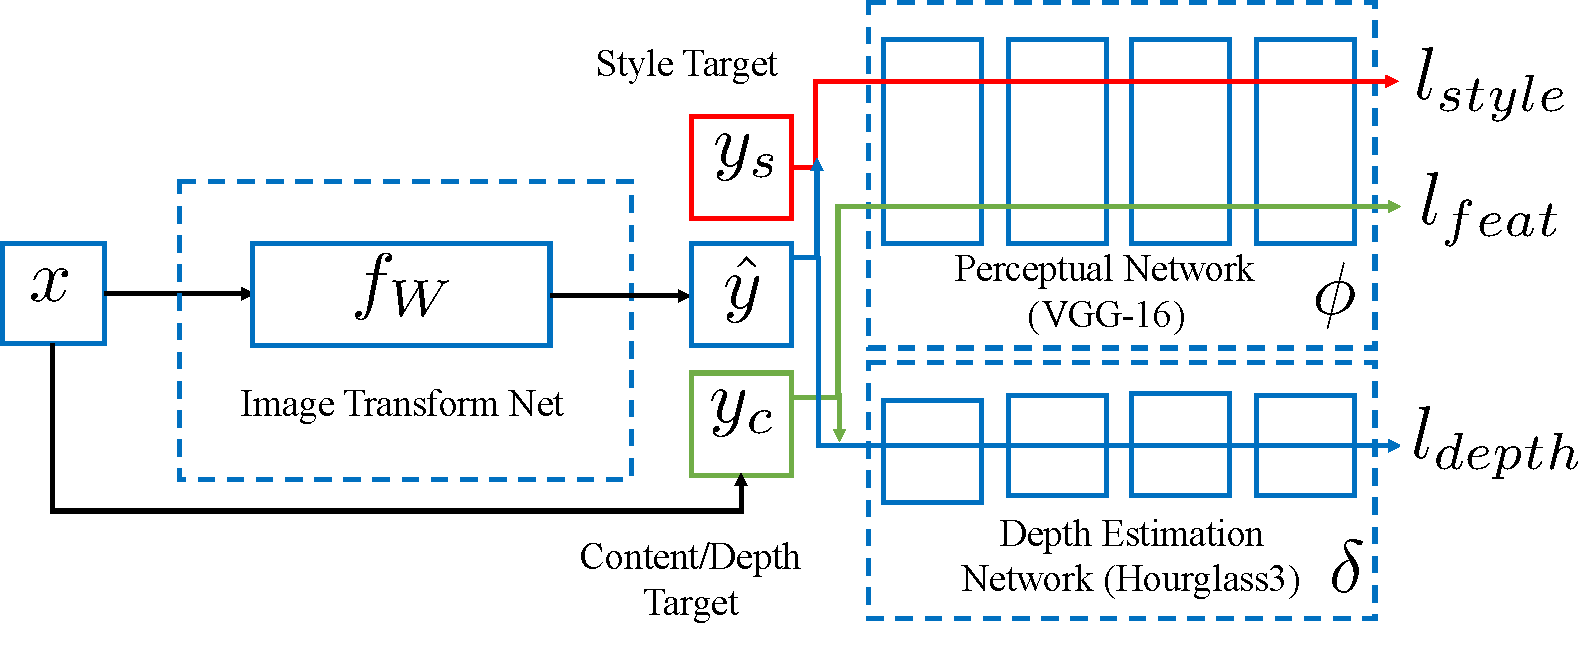
\includegraphics[scale=0.4]{network_structure.pdf}
\caption{Network Structure Overview}
\label{fig:overview}
\end{figure*}
The overview of our network structure is shown in Figure~\ref{fig:overview}. Compared to Johnson et al. \cite{johnson2016perceptual}'s work, our structure is featured in having a depth estimation network as part of our loss function. In all, our network is composed of 3 subnets: an image transformation network $f_W$, a perceptual loss network $\phi$ and a depth estimation network $\delta$. Similar to Johnson et al., the image transformation $f_W$ is a convolutional network which produce the output image $\hat y$ given the input image $x$ by $\hat y = f_W(x)$ (where $W$ is the weights of the network).

To keep track of the depth information, our loss function is composed of 2 neural networks: the perceptual loss network and the depth estimation network. As mentioned in \cite{johnson2016perceptual}, pretrained convolutional neural networks are able to extract perceptual information and encode semantics which are useful for the loss function. Similarly, a pretrained depth estimation network has already learned to estimate the depth information from the single input image. Therefore we utilize a pre-trained image classification network for the perceptual loss part and a pretrained depth estimation network for the depth loss part. Specifically, our loss function is defined as a weighted linear combination of the content loss $l_\text{content}$, the style loss $l_\text{style}$ and the depth loss $l_\text{depth}$. 

\[L(\hat y, y) = \lambda_1 l_\text{content}(\hat y, y) + \lambda_2 l_\text{style}(\hat y, y) + \lambda_3 l_\text{depth}(\hat y, y)\]

Therefore the training goal is to minimize the expected loss.

\[ W^* \gets \arg \min_W \mathbb E_{\{x,y\}}[L(f_W(x), y)], \]

%\begin{figure*}
\includepdf[pages=1, pagecommand=\subsection{blub}]{images.pdf}
%\end{figure*}

where $\mathbb E_{\{x,y\}}$ is the estimation of the expectation via the (training) set $\{x,y\}$.

\subsection{Depth Loss Function}

We make use of depth loss function to measure the amount of depth differences between the input image $x$ and the output image $\hat y$. Ideally, the output image should have similar depth features with that of the input. Rather than capture the per-pixel differences of the feed-forward outputs we capture the high level features from the depth estimation network. More specifically, we define the depth loss function $l_\text{depth}$ as the 2-norm of the feature vectors (from selected layers) \[l_\text{depth}(\hat y, y) = \sum_{i \in I_\delta} \frac{1}{N_i (\delta)}\|\delta_i(\hat y) - \delta_i(y)\|_2^2\], where $N_i(\delta)$ is the normalizing factor for the $i$-th layer in $\delta$ and $\delta_i(y)$ indicates the feature vector on the $i$-th layer if $y$ is feeded as the input to the network $\delta$. The layer set $I_\delta$ means the set of (high-level) layers we want to extract features from. The motivation for a high level depth loss function is that we want to encourage the output from $f_W$ to be similar to the content image from the depth pespective but we don't want their depth estimation to be exactly the same. There are several reasons for such a motivation: firstly, the estimations of depth from the network $\phi$ are not necessarily accurate which make it meaningless to pursue a (per-pixel) exact match on the depth estimation. Secondly, we need to allow the image transformatin network $f_W$ to perceptually transform the image which might involve changes of shapes, places and lines. Again it is not promising to propose a per-pixel loss, which reduce the chances of such transformations. Thirdly, as argued in \cite{johnson2016perceptual}, perceptual losses are more robust and stable than the per-pixel losses.

\subsection{Content Feature Loss Function and Style Loss Function}
For content feature loss function $l_\text{feat}$ and the style loss function $l_\text{style}$, we briefly recall the explanation from \cite{johnson2016perceptual}. As one of the main contributions in Johnson et al.'s paper, $l_\text{feat}$ and $l_\text{style}$ are both measures of differences of high-level features. $l_\text{feat}$ captures the distances in respect of perceptual features between the content target $y_c$(i.e., the input image $x$) and the output image $\hat y$. Similarly, as proposed from Gatys et al. \cite{gatys2016image}, $l_\text{style}$ captures the distances between the style image $y_s$ and the output image $\hat y$. 
%Though there are many options to quantify the distances, we simply adopt the 2-norm for the feature vectors. 
Therefore
\[ l_\text{feat}(\hat y, y) = \sum_{i \in I_\phi} \frac{1}{N_i(\phi)}\|\phi_i(\hat y) - \phi_i(y)\|_2^2, \]
and for style loss we use the Frobenius norm of differences of the Gram matrices of $\hat y$ and $y_s$.
\[ l_\text{style}(\hat y, y_s) = \sum_{i \in I_\phi} \frac{1}{N_i(\phi)}\|G^\phi_i(\hat y) - G^\phi_i(y_s)\|_F^2. \]
\section{Experiments}

\subsection{Training Details}

Microsoft COCO dataset~\cite{lin2014microsoft} (contiaing around 80K images) was used for training our depth-preserving style transfer networks. Each training image was resized to $256\times256$. Maximum iterations were set to be $40000$, and a batch size of 3 was applied. These settings gave roughly 1.5 epochs over all the training data. The optimization was based on Adam~\cite{kingma2014adam} with a learning rate of $1\times10^{-3}$. No weight decay or dropout was used. The training was implemented using Torch~\cite{collobert2011torch7} and cuDNN~\cite{chetlur2014cudnn}. Each style training took around 7 hours on a single GTX Titan X GPU. As for the target losses, the content target loss is computed at VGG network layer $relu2\_2$, the style target loss is computed at VGG network layers $relu1\_2$, $relu2\_2$, $relu3\_3$ and $relu4\_3$, and the depth target loss is computed at the output layer of Chen \etal network~\cite{chen2016single}.


\subsection{Qualitative Results}
In this section we present some results regarding the quality of our outputs. Generally, Structural Similarity Index is a method to measure the similarity between 2 images. It can be seen as a quality measure if the other image is considered truth (or perfect). For our case, we need to calculate the index between the original input and style transfered images. We measured the Structural Similarity Index against the original input of our results and the results from Johnson et al. \cite{johnson2016perceptual} on all the input images we tested with the style files provided by \cite{johnson2016perceptual}.
As shown in Figure~\ref{fig:ssim}, our results has a generally higher Structural Similarity Index than those from \cite{johnson2016perceptual}, which indicates that our method preserved much more structural information.

\begin{figure*}
\centering
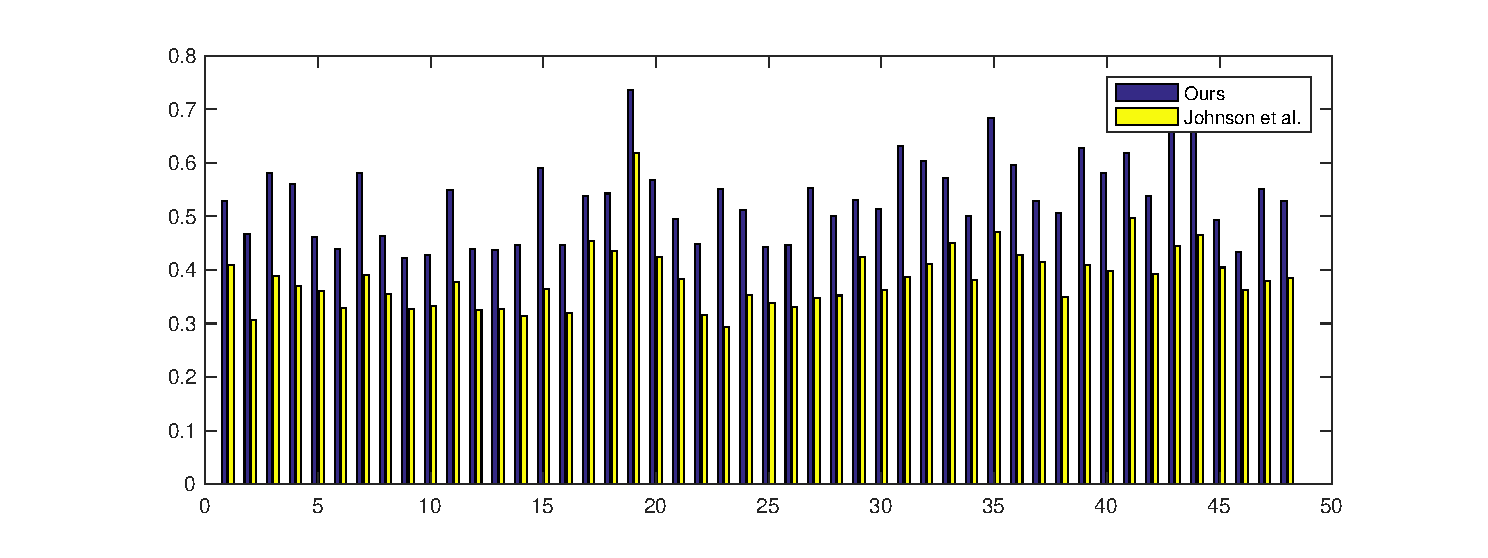
\includegraphics[scale=0.7]{ssim.eps}
\caption{Comparison of Structural Similarity Indices Against the Input Image Between Ours and Johnson et al. \cite{johnson2016perceptual}}
\label{fig:ssim}
\end{figure*}

\section{Discussion and Conlucsions}

Some might argue that if the weight for the style target loss in the Johnson \etal~\cite{johnson2016perceptual} network is decreased, we could get similar results. But this is not the case. Note that the content target loss term is computed as the distance of the feature representations in the VGG network~\cite{simonyan2014very}, which was designed and trained for object recognition. The backgrounds in the content images, for instance, skies, roads, and lawns, are hard to be fully represented in those features. Also, the depth of an ``object" (for example, the road in the teaser image) may change a lot in an image, and some pixel-level (or superpixel-level) loss should be included to preserve stereopsis of the transferred images. Therefore, an extra depth loss is necessitated in our problem setting.  

The intuition of why this depth loss net works is that style is put onto the content images layer by layer, not equally, when including the depth loss. As we can see from the outputs of Johnson \etal~\cite{johnson2016perceptual} network, the style is transferred almost equally to different regions of the content images. This may destruct stereopsis of the transferred images. The depth loss network we employed here, however, penalizes ``equal style transfer" across the content images.  

Some textures in our transferred images are also preserved as a by-product, for example, the rock texture and the grass texture in Figure~?. Again, this is due to that under the depth loss penalization, background features can be captured and preserved. This helps preserve textures of background objects.

In conclusion, the state-of-the-art work in style transfer~\cite{johnson2016perceptual} utilized the VGG network to capture perceptual features from content images, and they showed significant improvement of transfer speed compared to the previous work using pixel-level losses. However, the perceptual features extracted from layers in the VGG network can not fully represent background information. Especially, the depth of content images could not be preserved in some of their outputs. In this work, by combining the depth loss network with the perceptual losses, we demonstrated that our style transfer can preserve depth and stereopsis of the original content images, without losing the benefit of transferring speed. 

{\small
\bibliographystyle{ieee}
\bibliography{egbib}
}

\end{document}
